\documentclass[lualatex,handout]{beamer}
\setbeamertemplate{footline}[frame number]
\usepackage{luatexja}
\usepackage{amsmath,amssymb}

%\usetheme{Berlin}
\usecolortheme{rose}

\usepackage{tikz}
\usepackage{pgfplots}
\pgfplotsset{compat=1.18}

%\usepackage[haranoaji]{luatexja-preset}
\usepackage[deluxe,ipaex]{luatexja-preset}
\renewcommand{\kanjifamilydefault}{\gtdefault}
%\setmainjfont{HaranoAjiGothic-Regular}

\usepackage{unicode-math}
%\setmathfont{Fira Math}
\setmathfont{STIX Two Math}
\setmathrm{STIX Two Math}[StylisticSet=8]

%\usefonttheme{professionalfonts}

\usepackage{luacolor}

\newcommand{\emm}[1]{\textcolor{red}{#1}}
\newcommand{\expt}[1]{\mathbb{E}\left[#1\right]}
\newcommand{\var}[1]{\mathbb{V}\left[#1\right]}
\newcommand{\cov}[1]{\mathrm{Cov}\left[#1\right]}


\usepackage{xspace}
\newcommand\bm[1]{{\mathbf{#1}}}
\newcommand\dx{{\,\mathrm{d}x}}

\theoremstyle{definition}

\title{確率・統計基礎: 中心極限定理}
\author{森 立平}
\date{}



\begin{document}
\begin{frame}[plain]
\maketitle
\end{frame}

\begin{frame}{集中不等式}

確率変数$X_1,X_2,\dotsc,X_N$が\emm{独立}で\emm{同一の分布}に従うとき、
独立同分布(independently and identically distributed (i.i.d.))であるという。

\vspace{1em}
このスライドでは$X_1,\dotsc,X_N$は i.i.d.で確率変数$X$と同分布であると仮定する。

\vspace{1em}
\emm{$N$個のi.i.d.確率変数の平均$\frac{\sum_{k=1}^NX_k}{N}$が期待値$\expt{X}$周辺に集中}するというのが大数の法則や集中不等式が示すことである。
\end{frame}

\begin{frame}{二項分布}
\begin{align*}
\Pr(X = k) &= \binom{n}{k} p^k(1-p)^{n-k},\quad \emm{n=30},\, p=0.3.
\end{align*}
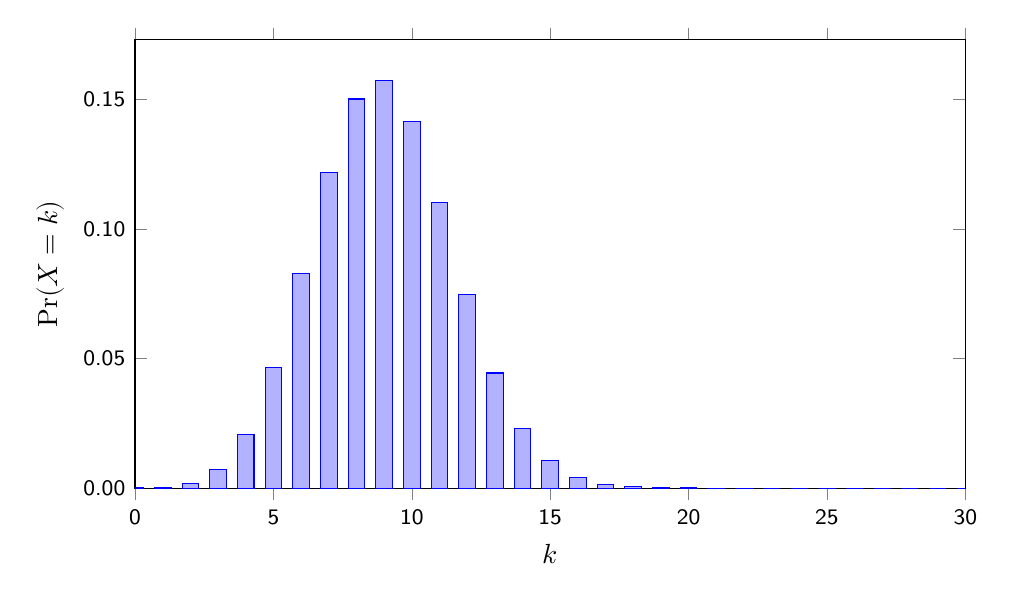
\begin{tikzpicture}[%
declare function={binom(\k,\n,\p)=\n!/(\k!*(\n-\k)!)*\p^\k*(1-\p)^(\n-\k);}]
\pgfmathsetmacro{\binomN}{30}
\begin{axis}[
    width=\textwidth, height=\axisdefaultheight,
    ylabel={$\Pr(X=k)$},
    xlabel={$k$},
    xmin=0, xmax=\binomN,
    ymin=0,
    scaled ticks = false,
    tick label style={/pgf/number format/assume math mode=true, font=\footnotesize\sffamily},
    yticklabel style={/pgf/number format/.cd, fixed, fixed zerofill, precision=2},
        domain=0:\binomN,samples at={0,1,...,\binomN},
    mark options={scale=0.75, blue},
    ybar, bar width = 6pt
        ]
%\addplot[ycomb] {binom(x,\binomN,0.3)};
\addplot {binom(x,\binomN,0.3)};
\end{axis}
\end{tikzpicture}
\end{frame}

\begin{frame}{二項分布}
\begin{align*}
\Pr(X = k) &= \binom{n}{k} p^k(1-p)^{n-k},\quad \emm{n=60},\, p=0.3.
\end{align*}
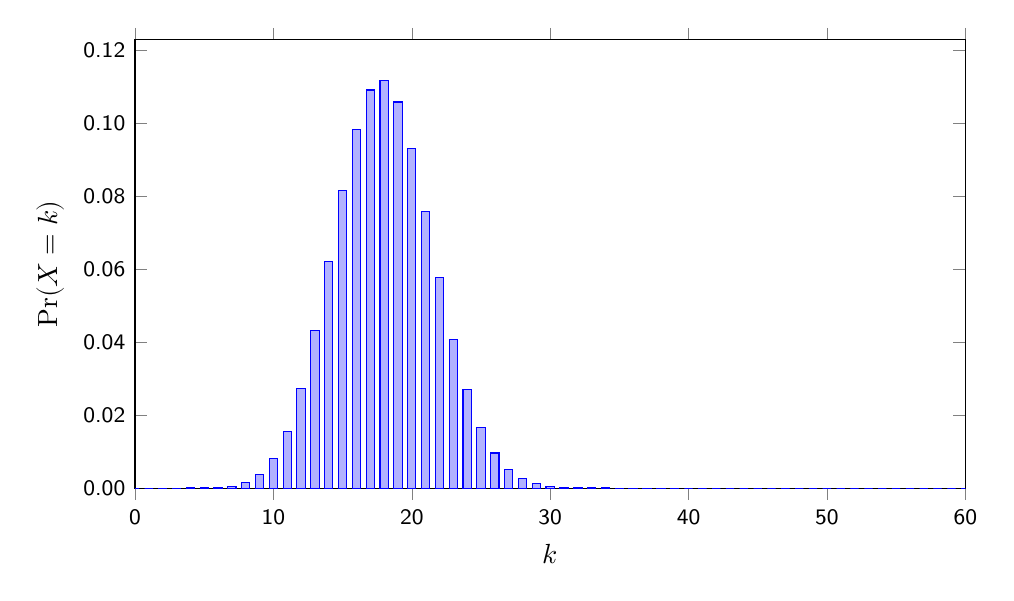
\begin{tikzpicture}[%
declare function={binom(\k,\n,\p)=\n!/(\k!*(\n-\k)!)*\p^\k*(1-\p)^(\n-\k);}]
\pgfmathsetmacro{\binomN}{60}
\begin{axis}[
    width=\textwidth, height=\axisdefaultheight,
    ylabel={$\Pr(X=k)$},
    xlabel={$k$},
    xmin=0, xmax=\binomN,
    ymin=0,
    scaled ticks = false,
    tick label style={/pgf/number format/assume math mode=true, font=\footnotesize\sffamily},
    yticklabel style={/pgf/number format/.cd, fixed, fixed zerofill, precision=2},
        domain=0:\binomN,samples at={0,1,...,\binomN},
    mark options={scale=0.75, blue},
    ybar, bar width = 3pt
        ]
%\addplot[ycomb] {binom(x,\binomN,0.3)};
\addplot {binom(x,\binomN,0.3)};
\end{axis}
\end{tikzpicture}
\end{frame}

\begin{frame}{二項分布}
\begin{align*}
\Pr(X = k) &= \binom{n}{k} p^k(1-p)^{n-k},\quad \emm{n=120},\, p=0.3.
\end{align*}
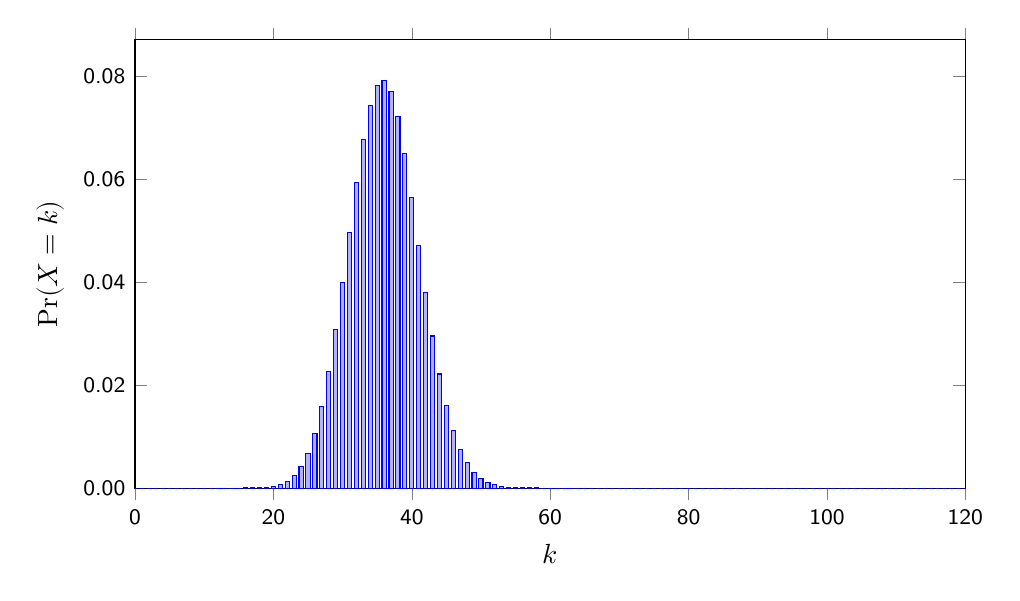
\begin{tikzpicture}[%
declare function={binom(\k,\n,\p)=\n!/(\k!*(\n-\k)!)*\p^\k*(1-\p)^(\n-\k);}]
\pgfmathsetmacro{\binomN}{120}
\begin{axis}[
    width=\textwidth, height=\axisdefaultheight,
    ylabel={$\Pr(X=k)$},
    xlabel={$k$},
    xmin=0, xmax=\binomN,
    ymin=0,
    scaled ticks = false,
    tick label style={/pgf/number format/assume math mode=true, font=\footnotesize\sffamily},
    yticklabel style={/pgf/number format/.cd, fixed, fixed zerofill, precision=2},
        domain=0:\binomN,samples at={0,1,...,\binomN},
    mark options={scale=0.75, blue},
    ybar, bar width = 1.5pt
        ]
%\addplot[ycomb] {binom(x,\binomN,0.3)};
\addplot {binom(x,\binomN,0.3)};
\end{axis}
\end{tikzpicture}
\end{frame}

\begin{frame}{二項分布}
\begin{align*}
\Pr(X = k) &= \binom{n}{k} p^k(1-p)^{n-k},\quad \emm{n=240},\, p=0.3.
\end{align*}
\begin{tikzpicture}[%
declare function={binom(\k,\n,\p)=\n!/(\k!*(\n-\k)!)*\p^\k*(1-\p)^(\n-\k);}]
\pgfmathsetmacro{\binomN}{240}
\pgfmathsetmacro{\p}{0.3}
\begin{axis}[
    width=\textwidth, height=\axisdefaultheight,
    ylabel={$\Pr(X=k)$},
    xlabel={$k$},
    xmin=0, xmax=\binomN,
    ymin=0,
    scaled ticks = false,
    tick label style={/pgf/number format/assume math mode=true, font=\footnotesize\sffamily},
    yticklabel style={/pgf/number format/.cd, fixed, fixed zerofill, precision=2},
        domain=0:\binomN,samples at={0,1,...,\binomN},
    mark options={scale=0.75, blue},
    ybar, bar width = .75pt
        ]
%\addplot[ycomb] {binom(x,\binomN,0.3)};
%\addplot {binom(x,\binomN,0.3)};
\addplot[domain=0:\binomN, color=blue, samples={\binomN+1}, thick] gnuplot { exp(lgamma(\binomN+1) - lgamma(x+1) - lgamma(\binomN-x+1) + x*log(\p) + (\binomN-x)*log(1-\p)) with impulses};
\end{axis}
\end{tikzpicture}
\end{frame}

\begin{frame}{二項分布}
\begin{align*}
\Pr(X = k) &= \binom{n}{k} p^k(1-p)^{n-k},\quad \emm{n=480},\, p=0.3.
\end{align*}
\begin{tikzpicture}[%
declare function={binom(\k,\n,\p)=\n!/(\k!*(\n-\k)!)*\p^\k*(1-\p)^(\n-\k);}]
\pgfmathsetmacro{\binomN}{480}
\pgfmathsetmacro{\p}{0.3}
\begin{axis}[
    width=\textwidth, height=\axisdefaultheight,
    ylabel={$\Pr(X=k)$},
    xlabel={$k$},
    xmin=0, xmax=\binomN,
    ymin=0,
    scaled ticks = false,
    tick label style={/pgf/number format/assume math mode=true, font=\footnotesize\sffamily},
    yticklabel style={/pgf/number format/.cd, fixed, fixed zerofill, precision=2},
        domain=0:\binomN,samples at={0,1,...,\binomN},
    mark options={scale=0.75, blue},
    ybar, bar width = .375pt
        ]
%\addplot[ycomb] {binom(x,\binomN,0.3)};
%\addplot {binom(x,\binomN,0.3)};
\addplot[domain=0:\binomN, color=blue, samples={\binomN+1}, thick] gnuplot { exp(lgamma(\binomN+1) - lgamma(x+1) - lgamma(\binomN-x+1) + x*log(\p) + (\binomN-x)*log(1-\p)) with impulses};
%\addplot[domain=0:\binomN, thick] gnuplot {x};
\end{axis}
\end{tikzpicture}
\end{frame}

\begin{frame}{二項分布}
\begin{align*}
\Pr(X = k) &= \binom{n}{k} p^k(1-p)^{n-k},\quad \emm{n=1000},\, p=0.3.
\end{align*}
\begin{tikzpicture}[%
declare function={binom(\k,\n,\p)=\n!/(\k!*(\n-\k)!)*\p^\k*(1-\p)^(\n-\k);}]
\pgfmathsetmacro{\binomN}{1000}
\pgfmathsetmacro{\p}{0.3}
\begin{axis}[
    width=\textwidth, height=\axisdefaultheight,
    ylabel={$\Pr(X=k)$},
    xlabel={$k$},
    xmin=0, xmax=\binomN,
    ymin=0,
    scaled ticks = false,
    tick label style={/pgf/number format/assume math mode=true, font=\footnotesize\sffamily},
    yticklabel style={/pgf/number format/.cd, fixed, fixed zerofill, precision=2},
        domain=0:\binomN,samples at={0,1,...,\binomN},
    mark options={scale=0.75, blue},
    ybar, bar width = .375pt
        ]
%\addplot[ycomb] {binom(x,\binomN,0.3)};
%\addplot {binom(x,\binomN,0.3)};
\addplot[domain=0:\binomN, color=blue, samples={\binomN+1}, thick] gnuplot { exp(lgamma(\binomN+1) - lgamma(x+1) - lgamma(\binomN-x+1) + x*log(\p) + (\binomN-x)*log(1-\p)) with impulses};
%\addplot[domain=0:\binomN, thick] gnuplot {x};
\end{axis}
\end{tikzpicture}
\end{frame}

\begin{frame}{二項分布}
\begin{align*}
\Pr(X = k) &= \binom{n}{k} p^k(1-p)^{n-k},\quad \emm{n=10000},\, p=0.3.
\end{align*}
\begin{tikzpicture}[%
declare function={binom(\k,\n,\p)=\n!/(\k!*(\n-\k)!)*\p^\k*(1-\p)^(\n-\k);}]
\pgfmathsetmacro{\binomN}{10000}
\pgfmathsetmacro{\p}{0.3}
\begin{axis}[
    width=\textwidth, height=\axisdefaultheight,
    ylabel={$\Pr(X=k)$},
    xlabel={$k$},
    xmin=0, xmax=\binomN,
    ymin=0,
    scaled ticks = false,
    tick label style={/pgf/number format/assume math mode=true, font=\footnotesize\sffamily},
    yticklabel style={/pgf/number format/.cd, fixed, fixed zerofill, precision=3},
        domain=0:\binomN,samples at={0,1,...,\binomN},
    mark options={scale=0.75, blue},
    ybar, bar width = .375pt
        ]
%\addplot[ycomb] {binom(x,\binomN,0.3)};
%\addplot {binom(x,\binomN,0.3)};
\addplot[domain=0:\binomN, color=blue, samples={\binomN+1}, thick] gnuplot { exp(lgamma(\binomN+1) - lgamma(x+1) - lgamma(\binomN-x+1) + x*log(\p) + (\binomN-x)*log(1-\p)) with impulses};
%\addplot[domain=0:\binomN, thick] gnuplot {x};
\end{axis}
\end{tikzpicture}
\end{frame}

\if0
\begin{frame}{二項分布}
\begin{align*}
\Pr(X = k) &= \binom{n}{k} p^k(1-p)^{n-k},\quad \emm{n=20000},\, p=0.3.
\end{align*}
\begin{tikzpicture}[%
declare function={binom(\k,\n,\p)=\n!/(\k!*(\n-\k)!)*\p^\k*(1-\p)^(\n-\k);}]
\pgfmathsetmacro{\binomN}{20000}
\pgfmathsetmacro{\p}{0.3}
\begin{axis}[
    width=\textwidth, height=\axisdefaultheight,
    ylabel={$\Pr(X=k)$},
    xlabel={$k$},
    xmin=0, xmax=\binomN,
    ymin=0,
    scaled ticks = false,
    tick label style={/pgf/number format/assume math mode=true, font=\footnotesize\sffamily},
    yticklabel style={/pgf/number format/.cd, fixed, fixed zerofill, precision=2},
        domain=0:\binomN,samples at={0,1,...,\binomN},
    mark options={scale=0.75, blue},
    ybar, bar width = .375pt
        ]
%\addplot[ycomb] {binom(x,\binomN,0.3)};
%\addplot {binom(x,\binomN,0.3)};
\addplot[domain=0:\binomN, color=blue, samples={\binomN+1}, thick] gnuplot { exp(lgamma(\binomN+1) - lgamma(x+1) - lgamma(\binomN-x+1) + x*log(\p) + (\binomN-x)*log(1-\p)) with impulses};
%\addplot[domain=0:\binomN, thick] gnuplot {x};
\end{axis}
\end{tikzpicture}
\end{frame}
\fi

\begin{frame}{二項分布}
\begin{align*}
\Pr(X = k) &= \binom{n}{k} p^k(1-p)^{n-k},\quad \emm{n=30},\, p=0.3.
\end{align*}
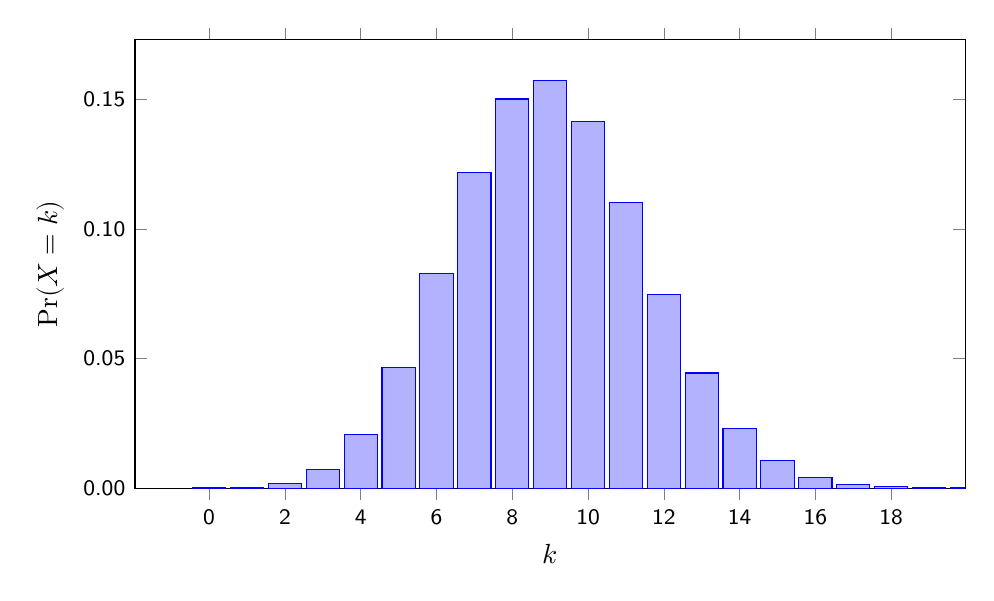
\begin{tikzpicture}[%
declare function={binom(\k,\n,\p)=\n!/(\k!*(\n-\k)!)*\p^\k*(1-\p)^(\n-\k);}]
\pgfmathsetmacro{\binomN}{30}
\pgfmathsetmacro{\p}{0.3}
\pgfmathsetmacro{\expect}{{\p*\binomN}}
\pgfmathsetmacro{\deviat}{{2*sqrt(\binomN)}}
\begin{axis}[
    width=\textwidth, height=\axisdefaultheight,
    ylabel={$\Pr(X=k)$},
    xlabel={$k$},
    xmin={\expect-\deviat}, xmax={\expect+\deviat},
    ymin=0,
    scaled ticks = false,
    tick label style={/pgf/number format/assume math mode=true, font=\footnotesize\sffamily},
    yticklabel style={/pgf/number format/.cd, fixed, fixed zerofill, precision=2},
        domain=0:\binomN,samples at={0,1,...,\binomN},
    mark options={scale=0.75, blue},
    ybar, bar width = 12pt
        ]
%\addplot[ycomb] {binom(x,\binomN,0.3)};
\addplot {binom(x,\binomN,\p)};
\end{axis}
\end{tikzpicture}
\end{frame}

\begin{frame}{二項分布}
\begin{align*}
\Pr(X = k) &= \binom{n}{k} p^k(1-p)^{n-k},\quad \emm{n=60},\, p=0.3.
\end{align*}
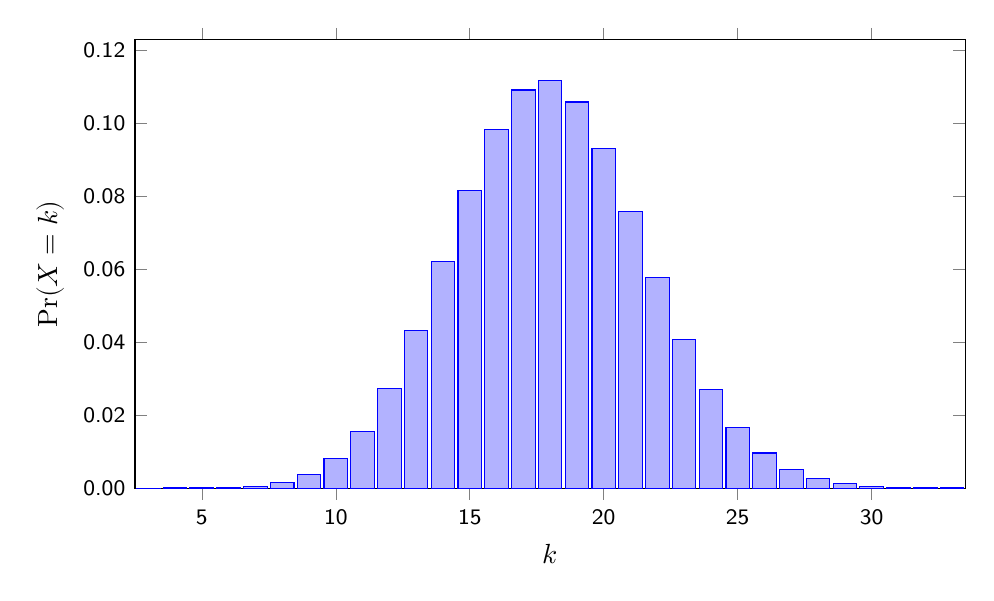
\begin{tikzpicture}[%
declare function={binom(\k,\n,\p)=\n!/(\k!*(\n-\k)!)*\p^\k*(1-\p)^(\n-\k);}]
\pgfmathsetmacro{\binomN}{60}
\pgfmathsetmacro{\p}{0.3}
\pgfmathsetmacro{\expect}{{\p*\binomN}}
\pgfmathsetmacro{\deviat}{{2*sqrt(\binomN)}}
\begin{axis}[
    width=\textwidth, height=\axisdefaultheight,
    ylabel={$\Pr(X=k)$},
    xlabel={$k$},
    xmin={\expect-\deviat}, xmax={\expect+\deviat},
    ymin=0,
    scaled ticks = false,
    tick label style={/pgf/number format/assume math mode=true, font=\footnotesize\sffamily},
    yticklabel style={/pgf/number format/.cd, fixed, fixed zerofill, precision=2},
        domain=0:\binomN,samples at={0,1,...,\binomN},
    mark options={scale=0.75, blue},
    ybar, bar width = 8.5pt
        ]
%\addplot[ycomb] {binom(x,\binomN,0.3)};
\addplot {binom(x,\binomN,\p)};
\end{axis}
\end{tikzpicture}
\end{frame}

\begin{frame}{二項分布}
\begin{align*}
\Pr(X = k) &= \binom{n}{k} p^k(1-p)^{n-k},\quad \emm{n=120},\, p=0.3.
\end{align*}
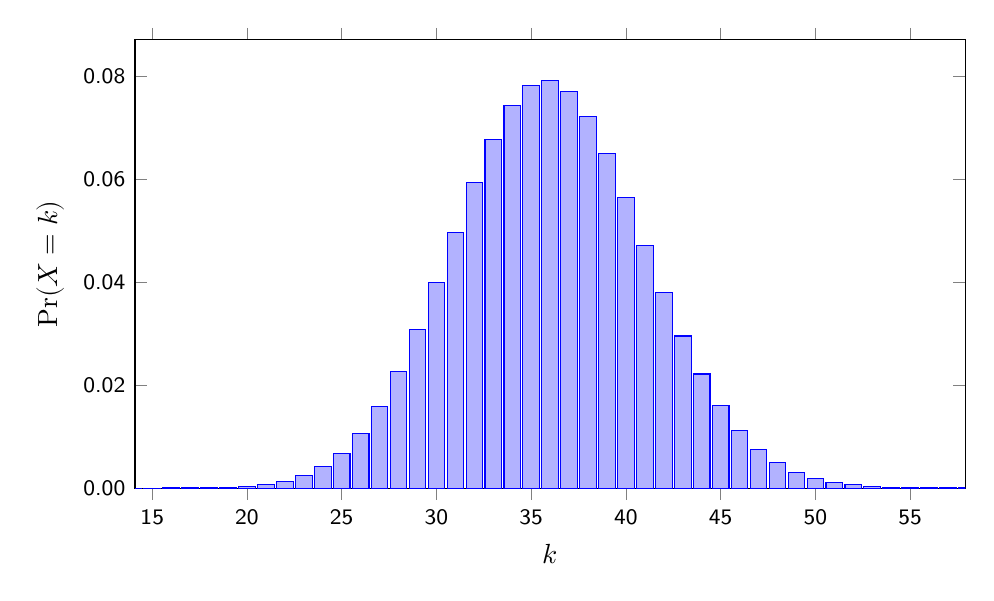
\begin{tikzpicture}[%
declare function={binom(\k,\n,\p)=\n!/(\k!*(\n-\k)!)*\p^\k*(1-\p)^(\n-\k);}]
\pgfmathsetmacro{\binomN}{120}
\pgfmathsetmacro{\p}{0.3}
\pgfmathsetmacro{\expect}{{\p*\binomN}}
\pgfmathsetmacro{\deviat}{{2*sqrt(\binomN)}}
\begin{axis}[
    width=\textwidth, height=\axisdefaultheight,
    ylabel={$\Pr(X=k)$},
    xlabel={$k$},
    xmin={\expect-\deviat}, xmax={\expect+\deviat},
    ymin=0,
    scaled ticks = false,
    tick label style={/pgf/number format/assume math mode=true, font=\footnotesize\sffamily},
    yticklabel style={/pgf/number format/.cd, fixed, fixed zerofill, precision=2},
        domain=0:\binomN,samples at={0,1,...,\binomN},
    mark options={scale=0.75, blue},
    ybar, bar width = 6pt
        ]
%\addplot[ycomb] {binom(x,\binomN,0.3)};
\addplot {binom(x,\binomN,\p)};
\end{axis}
\end{tikzpicture}
\end{frame}

\begin{frame}{二項分布}
\begin{align*}
\Pr(X = k) &= \binom{n}{k} p^k(1-p)^{n-k},\quad \emm{n=240},\, p=0.3.
\end{align*}
\begin{tikzpicture}[%
declare function={binom(\k,\n,\p)=\n!/(\k!*(\n-\k)!)*\p^\k*(1-\p)^(\n-\k);}]
\pgfmathsetmacro{\binomN}{240}
\pgfmathsetmacro{\p}{0.3}
\pgfmathsetmacro{\expect}{{\p*\binomN}}
\pgfmathsetmacro{\deviat}{{2*sqrt(\binomN)}}
\begin{axis}[
    width=\textwidth, height=\axisdefaultheight,
    ylabel={$\Pr(X=k)$},
    xlabel={$k$},
    xmin={\expect-\deviat}, xmax={\expect+\deviat},
    ymin=0,
    scaled ticks = false,
    tick label style={/pgf/number format/assume math mode=true, font=\footnotesize\sffamily},
    yticklabel style={/pgf/number format/.cd, fixed, fixed zerofill, precision=2},
        domain=0:\binomN,samples at={0,1,...,\binomN},
    mark options={scale=0.75, blue},
    ybar, bar width = 4.25pt
        ]
%\addplot[ycomb] {binom(x,\binomN,0.3)};
%\addplot {binom(x,\binomN,\p)};
\addplot[domain=0:\binomN, color=blue, samples={\binomN+1}, thick] gnuplot { exp(lgamma(\binomN+1) - lgamma(x+1) - lgamma(\binomN-x+1) + x*log(\p) + (\binomN-x)*log(1-\p)) with impulses};
\end{axis}
\end{tikzpicture}
\end{frame}

\begin{frame}{二項分布}
\begin{align*}
\Pr(X = k) &= \binom{n}{k} p^k(1-p)^{n-k},\quad \emm{n=480},\, p=0.3.
\end{align*}
\begin{tikzpicture}[%
declare function={binom(\k,\n,\p)=\n!/(\k!*(\n-\k)!)*\p^\k*(1-\p)^(\n-\k);}]
\pgfmathsetmacro{\binomN}{480}
\pgfmathsetmacro{\p}{0.3}
\pgfmathsetmacro{\expect}{{\p*\binomN}}
\pgfmathsetmacro{\deviat}{{2*sqrt(\binomN)}}
\begin{axis}[
    width=\textwidth, height=\axisdefaultheight,
    ylabel={$\Pr(X=k)$},
    xlabel={$k$},
    xmin={\expect-\deviat}, xmax={\expect+\deviat},
    ymin=0,
    scaled ticks = false,
    tick label style={/pgf/number format/assume math mode=true, font=\footnotesize\sffamily},
    yticklabel style={/pgf/number format/.cd, fixed, fixed zerofill, precision=2},
        domain=0:\binomN,samples at={0,1,...,\binomN},
    mark options={scale=0.75, blue},
    ybar, bar width = 3pt
        ]
%\addplot[ycomb] {binom(x,\binomN,0.3)};
%\addplot {binom(x,\binomN,\p)};
%\addplot[domain={\expect-\deviat}:{\expect+\deviat}, color=blue, samples={2*\deviat+1}, thick] gnuplot { exp(lgamma(\binomN+1) - lgamma(x+1) - lgamma(\binomN-x+1) + x*log(\p) + (\binomN-x)*log(1-\p)) with impulses};
\addplot[domain=0:\binomN, color=blue, samples={\binomN+1}, thick] gnuplot { exp(lgamma(\binomN+1) - lgamma(x+1) - lgamma(\binomN-x+1) + x*log(\p) + (\binomN-x)*log(1-\p)) with impulses};
\end{axis}
\end{tikzpicture}
\end{frame}

\begin{frame}{二項分布}
\begin{align*}
\Pr(X = k) &= \binom{n}{k} p^k(1-p)^{n-k},\quad \emm{n=1000},\, p=0.3.
\end{align*}
\begin{tikzpicture}[%
declare function={binom(\k,\n,\p)=\n!/(\k!*(\n-\k)!)*\p^\k*(1-\p)^(\n-\k);}]
\pgfmathsetmacro{\binomN}{1000}
\pgfmathsetmacro{\p}{0.3}
\pgfmathsetmacro{\expect}{{\p*\binomN}}
\pgfmathsetmacro{\deviat}{{2*sqrt(\binomN)}}
\begin{axis}[
    width=\textwidth, height=\axisdefaultheight,
    ylabel={$\Pr(X=k)$},
    xlabel={$k$},
    xmin={\expect-\deviat}, xmax={\expect+\deviat},
    ymin=0,
    scaled ticks = false,
    tick label style={/pgf/number format/assume math mode=true, font=\footnotesize\sffamily},
    yticklabel style={/pgf/number format/.cd, fixed, fixed zerofill, precision=2},
        domain=0:\binomN,samples at={0,1,...,\binomN},
    mark options={scale=0.75, blue},
    ybar, bar width = 2pt
        ]
%\addplot[ycomb] {binom(x,\binomN,0.3)};
%\addplot {binom(x,\binomN,\p)};
%\addplot[domain={\expect-\deviat}:{\expect+\deviat}, color=blue, samples={2*\deviat+1}, thick] gnuplot { exp(lgamma(\binomN+1) - lgamma(x+1) - lgamma(\binomN-x+1) + x*log(\p) + (\binomN-x)*log(1-\p)) with impulses};
\addplot[domain=0:\binomN, color=blue, samples={\binomN+1}, thick] gnuplot { exp(lgamma(\binomN+1) - lgamma(x+1) - lgamma(\binomN-x+1) + x*log(\p) + (\binomN-x)*log(1-\p)) with impulses};
\end{axis}
\end{tikzpicture}
\end{frame}

\begin{frame}{二項分布}
\begin{align*}
\Pr(X = k) &= \binom{n}{k} p^k(1-p)^{n-k},\quad \emm{n=10000},\, p=0.3.
\end{align*}
\begin{tikzpicture}[%
declare function={binom(\k,\n,\p)=\n!/(\k!*(\n-\k)!)*\p^\k*(1-\p)^(\n-\k);}]
\pgfmathsetmacro{\binomN}{10000}
\pgfmathsetmacro{\p}{0.3}
\pgfmathsetmacro{\expect}{{\p*\binomN}}
\pgfmathsetmacro{\deviat}{{2*sqrt(\binomN)}}
\begin{axis}[
    width=\textwidth, height=\axisdefaultheight,
    ylabel={$\Pr(X=k)$},
    xlabel={$k$},
    xmin={\expect-\deviat}, xmax={\expect+\deviat},
    ymin=0,
    scaled ticks = false,
    tick label style={/pgf/number format/assume math mode=true, font=\footnotesize\sffamily},
    yticklabel style={/pgf/number format/.cd, fixed, fixed zerofill, precision=3},
        domain=0:\binomN,samples at={0,1,...,\binomN},
    mark options={scale=0.75, blue},
    ybar, bar width = .4pt
        ]
%\addplot[ycomb] {binom(x,\binomN,0.3)};
%\addplot {binom(x,\binomN,\p)};
%\addplot[domain={\expect-\deviat}:{\expect+\deviat}, color=blue, samples={2*\deviat+1}, thick] gnuplot { exp(lgamma(\binomN+1) - lgamma(x+1) - lgamma(\binomN-x+1) + x*log(\p) + (\binomN-x)*log(1-\p)) with impulses};
\addplot[domain=0:\binomN, color=blue, samples={\binomN+1}, thick] gnuplot { exp(lgamma(\binomN+1) - lgamma(x+1) - lgamma(\binomN-x+1) + x*log(\p) + (\binomN-x)*log(1-\p)) with impulses};
\end{axis}
\end{tikzpicture}
\end{frame}

\if0
\begin{frame}{二項分布}
\begin{align*}
\Pr(X = k) &= \binom{n}{k} p^k(1-p)^{n-k},\quad \emm{n=10000},\, p=0.3.
\end{align*}
\begin{tikzpicture}[%
declare function={binom(\k,\n,\p)=\n!/(\k!*(\n-\k)!)*\p^\k*(1-\p)^(\n-\k);}]
\pgfmathsetmacro{\binomN}{10000}
\pgfmathsetmacro{\p}{0.3}
\pgfmathsetmacro{\expect}{{\p*\binomN}}
\pgfmathsetmacro{\deviat}{{sqrt(\binomN)}}
\begin{axis}[
    width=\textwidth, height=\axisdefaultheight,
    ylabel={$\Pr(X=k)$},
    xlabel={$k$},
    xmin={\expect-\deviat}, xmax={\expect+\deviat},
    ymin=0,
    scaled ticks = false,
    tick label style={/pgf/number format/assume math mode=true, font=\footnotesize\sffamily},
    yticklabel style={/pgf/number format/.cd, fixed, fixed zerofill, precision=3},
        domain=0:\binomN,samples at={0,1,...,\binomN},
    mark options={scale=0.75, blue},
    ybar, bar width = .4pt
        ]
%\addplot[ycomb] {binom(x,\binomN,0.3)};
%\addplot {binom(x,\binomN,\p)};
%\addplot[domain={\expect-\deviat}:{\expect+\deviat}, color=blue, samples={2*\deviat+1}, thick] gnuplot { exp(lgamma(\binomN+1) - lgamma(x+1) - lgamma(\binomN-x+1) + x*log(\p) + (\binomN-x)*log(1-\p)) with impulses};
\addplot[domain=0:\binomN, color=blue, samples={\binomN+1}, thick] gnuplot { exp(lgamma(\binomN+1) - lgamma(x+1) - lgamma(\binomN-x+1) + x*log(\p) + (\binomN-x)*log(1-\p)) with impulses};
%\addplot {exp(-(x-\expect)^2/(2*sqrt(\binomN)))};
\end{axis}
\end{tikzpicture}
\end{frame}
\fi

\begin{frame}{中心極限定理}
\small
\begin{theorem}[中心極限定理]
$X$が分散を持つと仮定する。
\begin{align*}
\lim_{N\to\infty}\Pr\left(\frac{\left(\sum_{k=1}^N X_k\right)-N\expt{X}}{\sqrt{\var{X}N}} \le x\right) &= \Phi(x)
=\frac1{\sqrt{2\pi}}\int_{-\infty}^x\mathrm{e}^{-\frac{t^2}2}\mathrm{d}t
\end{align*}
\end{theorem}
\begin{align*}
Y_k&:= \frac{X_k-\expt{X}}{\sqrt{\var{X}}}\qquad \text{for } k=1,2,\dotsc,N
\end{align*}
は平均0、分散1に正規化した確率変数である。
中心極限定理の主張は
\begin{align*}
\lim_{N\to\infty}\Pr\left(\frac{\sum_{k=1}^N Y_k}{\sqrt{N}} \le x\right) &= \Phi(x)
\end{align*}
である。$N$で割るのではなくて$\sqrt{N}$で割ることで大数の法則よりも細かい部分を見ている。
\end{frame}

\begin{frame}{特性関数}
\begin{definition}[特性関数]
確率変数$X$の\emm{特性関数}を以下で定義する。
\begin{align*}
\varphi_X(t) &:= \expt{\mathrm{e}^{itX}}.
\end{align*}
モーメント母関数は存在するとは限らないが特性関数は(定義域を$\mathbb{R}$として)常に存在する。

\vspace{.5em}
$X$が$k$次モーメントを持つ$\iff$$\varphi_X$は0で$k$回微分できる。
\begin{align*}
\left.\frac{\mathrm{d}^k\varphi_X(t)}{\mathrm{d}t^k}\right|_{t=0} &= i^k \expt{X^k}.
\end{align*}

\vspace{1em}
第二特性関数
\begin{align*}
H_X(t) &:= \log\expt{\mathrm{e}^{itX}}
\end{align*}
\end{definition}
\end{frame}

\begin{frame}{コーシー分布の特性関数}
\end{frame}

\begin{frame}{分布の収束と特性関数の収束}
\begin{theorem}
確率変数の列$Z_1,Z_2,\dotsc$と確率変数$Z$について
\begin{align*}
\lim_{n\to\infty}\varphi_{Z_n}(t) = \varphi_Z(t)\qquad\forall t\in\mathbb{R}
\end{align*}
のとき、
\begin{align*}
\lim_{n\to\infty} \Pr(Z_n\le x) &= \Pr(Z\le x)\qquad\forall x\in\mathbb{R}
\end{align*}
\end{theorem}
\end{frame}

\begin{frame}{中心極限定理の証明}
\small
平均0分散1のi.i.d.確率変数$Y_1,\dotsc,Y_N$と標準正規分布に従う確率変数$Z$について
\begin{align*}
\lim_{N\to\infty}\Pr\left(\frac{\sum_{k=1}^N Y_k}{\sqrt{N}} \le x\right) &= \Pr(Z\le x)
\end{align*}
を示す。

\begin{align*}
\lim_{N\to\infty} H_{\frac{\sum_kY_k}{\sqrt{N}}}(t) &= \varphi_Z(t) = -\frac{t^2}2
\end{align*}
を示せばよい。$Y$は分散を持つので$H_Y$は0で二階微分できる。
\begin{align*}
H_{\frac{\sum_kY_k}{\sqrt{N}}}(t) &= 
H_{\sum_kY_k}\left(\frac{t}{\sqrt{N}}\right)\\
&= NH_Y\left(\frac{t}{\sqrt{N}}\right)\\
&= N\left(H_Y(0) + H_Y'(0)\frac{t}{\sqrt{N}} + \frac{H_Y''(0)}2\left(\frac{t}{\sqrt{N}}\right)^2 + o\left(\frac{1}{N}\right)\right)
= -\frac{t^2}2
\end{align*}
\end{frame}

\begin{frame}{集中不等式との比較}
\begin{align*}
%\Pr\left(\frac1N\sum_{k=1}^N X_k\ge \expt{X} + \frac{a}{\sqrt{N}}\right) &\le \mathrm{e}^{-\frac{\left(a/\sqrt{N}\right)^2}{2s^2}N}
\Pr\left(\frac1N\sum_{k=1}^N X_k\ge \expt{X} + \frac{a}{\sqrt{N}}\right) &\le \mathrm{e}^{-I_X\left(\expt{X}+\frac{a}{\sqrt{N}}\right)N}
\approx \mathrm{e}^{-\frac{I_X''(\expt{X})}2 a^2}
= \mathrm{e}^{-\frac{a^2}{2\var{X}}}\\
\Pr\left(\frac1N\sum_{k=1}^N X_k\ge \expt{X} + \frac{a}{\sqrt{N}}\right) &\to 
%1-\Phi\left(\frac{a}{\sqrt{\var{X}}}\right)
\frac1{\sqrt{2\pi}}\int_{\frac{a}{\sqrt{\var{X}}}}^\infty \mathrm{e}^{-\frac{x^2}2}\dx
\end{align*}
\begin{align*}
I_X\left(\expt{X}+\frac{a}{\sqrt{N}}\right)&=I_X(\expt{X}) + I_X'(\expt{X})\frac{a}{\sqrt{N}} + \frac{I_X''(\expt{X})}2\frac{a^2}N + o\left(\frac1N\right)\\
&= \frac1{2\var{X}}\frac{a^2}N + o\left(\frac1N\right)
\end{align*}
\end{frame}

\end{document}
